%%%%%%%%%%%%%%%%%%%%%%%%%%%%%%%%%%%%%%%%%
% University/School Laboratory Report
% LaTeX Template
% Version 3.1 (25/3/14)
%
% This template has been downloaded from:
% http://www.LaTeXTemplates.com
%
% Original author:
% Linux and Unix Users Group at Virginia Tech Wiki 
% (https://vtluug.org/wiki/Example_LaTeX_chem_lab_report)
%
% License:
% CC BY-NC-SA 3.0 (http://creativecommons.org/licenses/by-nc-sa/3.0/)
%
%%%%%%%%%%%%%%%%%%%%%%%%%%%%%%%%%%%%%%%%%

%----------------------------------------------------------------------------------------
%	PACKAGES AND DOCUMENT CONFIGURATIONS
%----------------------------------------------------------------------------------------

\documentclass[UTF8]{ctexart}

\usepackage{siunitx} % Provides the \SI{}{} and \si{} command for typesetting SI units
\usepackage{graphicx} % Required for the inclusion of images
\usepackage{graphics} % 图片设置
\usepackage{subfigure} 

\usepackage{natbib} % Required to change bibliography style to APA
\usepackage{amsmath} % Required for some math elements 
\usepackage{amssymb} % 使用因为所以符号
\usepackage{fancyhdr} % 使用页眉

\usepackage{algorithm}
\usepackage{algorithmic}

\usepackage{listings} % 插入代码
\usepackage{xcolor}

\usepackage{enumerate} % 列表

\lstset{
    %backgroundcolor=\color{red!50!green!50!blue!50},%代码块背景色为浅灰色
    rulesepcolor= \color{gray}, %代码块边框颜色
    breaklines=true,  %代码过长则换行
    numbers=left, %行号在左侧显示
    numberstyle= \small,%行号字体
    %keywordstyle= \color{red},%关键字颜色
    commentstyle=\color{gray}, %注释颜色
    frame=shadowbox%用方框框住代码块
    }

%\usepackage{url} % 引用URL
% \usepackage{cite}
% \newcommand{\upcite}[1]{\textsuperscript{\textsuperscript{\cite{#1}}}} %参考文献上标
%\bibliographystyle{plain}   %引用的样式%

\pagestyle{fancy}
\fancyhf{} 
\cfoot{\thepage} 

\setlength\parindent{0pt} % Removes all indentation from paragraphs

\renewcommand{\labelenumi}{\alph{enumi}.} 

%----------------------------------------------------------------------------------------
%	DOCUMENT INFORMATION
%----------------------------------------------------------------------------------------
\title{算法分析与设计-作业七}

\author{王宸昊 2019214541}

\date{\today}

\begin{document}

\maketitle

%----------------------------------------------------------------------------------------
%	SECTION 1
%----------------------------------------------------------------------------------------

\section{CLRS, Page, 360 22.5-7}

\subsection{算法思想}

首先对有向图G(V, E)使用求强连通分量的算法,,然后对强连通分量进行收缩,形成无环分量图。再对此无环分量图进行拓扑排序,得到的顶点序列,如果依次存在边相连,则该有向图G是半连通的。

\subsection{算法伪代码}

\begin{algorithm}[H]
	\caption{IS-SEMI-CONNECTED(G)}  % 算法标题
    \begin{algorithmic}[1]  % 一行一个标行号
        \STATE Computer the component graph of G, called G'
        \STATE Call topological sort on G', get list of vertices $v_1, v_2, \dots, v_k$.
        \FOR{$i=0$ to $k-1$}
        \IF{no edge between $v_i$ and $v_{i+1}$}
        \RETURN{FALSE}
        \ENDIF
        \ENDFOR
        \RETURN{TRUE}
	\end{algorithmic}
\end{algorithm}

 \subsection{正确性证明}

 假设图G中的任意两个顶点$v_i, v_j$.\\
 当$v_i, v_j$属于同一个强连通分量时,则一定满足半连通的条件。\\
 当$v_i, v_j$不属于同一个强连通分量时,则在对应的无环连通图中,属于不同的顶点,当进行拓扑排序后,如果每个相邻的顶点都存在边,则一定一条路径使得$v_i$可以抵达$v_j$或者$v_j$可以抵达$v_i$,则此时图G是半连通的,否则则不存在$v_i$到$v_j$的边,即不连通。

 \subsection{复杂性分析}
 求强连通分量的时间复杂度为O(V+R),拓扑排序的时间复杂度为O(V+E),因此总的算法复杂度为O(V+E)。

%----------------------------------------------------------------------------------------
%	SECTION 2
%----------------------------------------------------------------------------------------

\section{CLRS, Page, 370 23.2-7}

假设图G(V, E)的最小生成树为T,最小生成树的边集为$E_T$,加入一个新顶点后的最小生成树为T',其相关的边集为$E_{add}$。由树的定义可以知道,树T中边的个数为$V.num-1$。\\
当新加入的结点只有一条边时,即更新后的最小生成树T'就是在T的基础上加上顶点和这条相关的边。
因为此时只有一条边可以抵达该结点,所以此时T'的边的权重一定是最小的。\\
当新加入的结点相关边为k时(k>1),则要在边集\{ $E_{T} \cup E_{add}$ \} 中删除k-1条边。具体删除的策略为对该顶点进行k-1次DFS,每次都能找到一条回路,然后删除回路中权值最大的一条边。\\

证明:该问题可以转化为添加新节点后的G',构成其最小生成树的边一定在之前的最小生成树的边集和添加的边集中,即在\{ $E_{T} \cup E_{add}$ \}中。假设加入新的点和相关的边后,最小生成树T变为了一个图G',此时的最小生成树为T',最小生成树的边集为$E_{T'} \subset \{E_{T} \cup E_{add}\}  $。

反证法:假如T'中的存在边 $e \subset E - \{E_{T} \cup E_{add}\}$,由于对于新加入节点之前的图G,由于G存在最小生成树T,T当中不存在边e,所以一定能找出一条比e权重更小的边,使得从起点到终点的权重小于e的两个端点,此时e不是最小生成树的边,所以假设不成立。\\

由于算法只对部分顶点进行了DFS,所以整体的算法复杂度为O(V+E).

%----------------------------------------------------------------------------------------
%	SECTION 3
%----------------------------------------------------------------------------------------

\section{CLRS, Page, 370 23-1}

\subsection{证明:次优最小生成树不唯一}
只要举出一个反例即可,如下无向图:
\begin{figure}[H]
    \centering
    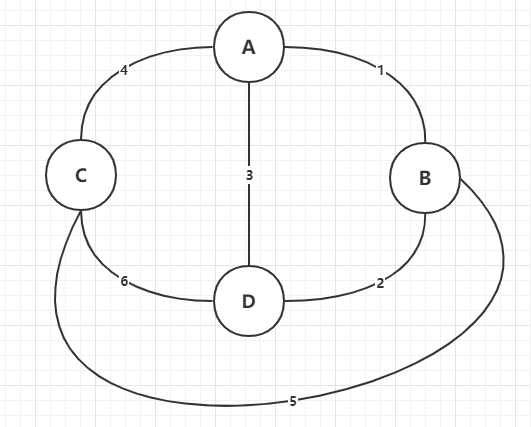
\includegraphics[width=1\textwidth]{img/img1.png}
    \caption{无向图}
    \label{img1}
\end{figure}
其最小生成树唯一,权重为7,边集为(a,b)(b,d)(a,c)\\
次优最小生成树有两个,权重为8,边集为(a,b)(a,d)(a,c)和(a,b)(a,d)(b,c)

\subsection{证明:次优生成树}
即证明次优生成树只是对最优生成树其中的一条边进行了替换。\\
反证法:假设最优生成树T和次优生成树T'存在两条以上不同的边,从T中挑选出一条不同的边,加入到T'当中,此时次优生成树构成了有环图,此时从次优生成树的边中删除一条边,此时构成的生成树T''与T只差一条边,由最优生成树的概念可知,此时三个树的权重关系为W(T) < W(T'') < W(T'),由此可见W(T')并不是次优最小生成树,所以假设不成立。

\subsection{设计算法计算max[u, v]}
采用dp的思想,假设(u,v)之间最大的权重的边的值为二维矩阵dp[u,v]的值,假设x是u直接相邻的节点,则状态转移方程为(u,v) = MAX(w(u, x), dp(x,v))\\

具体的实现可以使用从任意节点开始的BFS,记录max[u, v],由于需要记录整个max[V][V]的二维数组,所以复杂度为$O(V^2)$

\subsection{设计算法计算次优最小生成树}

1. 首先根据图G按照Kruskal或Prim算法生成最优生成树\\
2. 按照第三问的算法, 计算出最小生成树中的max矩阵\\
3. 遍历所有不在最小生成树当中的边e,使得w(e)-w(max[u,v])最小\\
4. 将e加入到最小生成树,并从T中删除max[u,v],此时得到的树即为次优最小生成树.\\

根据上述算法复杂度分析可知,最终的整体算法复杂度为$O(V^2)$。


%----------------------------------------------------------------------------------------
%	SECTION 4
%----------------------------------------------------------------------------------------

\section{CLRS, Page, 381 24.1-6}

\subsection{算法思想}

根据Bellman-Ford算法,假如存在负权重的环,则在对(u,v)进行遍历时,会产生v.d>u.d+w(u,v),返回False,则存在负权重的环路。\\
针对v进行DFS,如果搜索时,某一节点的前驱是灰色节点,说明该节点的前驱还未搜索完毕,即产生了环。\\
综合以上两种算法,则可以得到该负权重环上的所有节点

\subsection{伪代码}

\begin{lstlisting}
    BELLMAN-Ford(G, w, s)
        INITIALIZE-SINGLE-SOURCE(G, s)
        for i=1 to G.V-1
            for each edge(u,v) in G.E
                RELAX(u, v, w)
        for each edge(u,v) in G.E
            if v.d > u.d + w(u, v)
                DFS(v)
    
    DFS(v)
        if v.color == GRAY:
            return v
        if v.parent != NULL
            v.color = GRAY
            par = DFS(v.parent)
            v.color = black
            if par != NULL
                return v.append(par)

            return NULL
    \end{lstlisting}
\end{document}